%%%%%%%%%%%%%%%%%%%%%%%%%%%%%%%
%This is the article LaTeX template for RSC journals
%Copyright The Royal Society of Chemistry 2010
%%%%%%%%%%%%%%%%%%%%%%%%%%%%%%%


\documentclass[8.5pt,twoside,twocolumn]{article}
\oddsidemargin -1.2cm
\evensidemargin -1.2cm
\textwidth 18cm
\headheight 1.0in
\topmargin -3.5cm
\textheight 22cm
\usepackage[super,sort&compress,comma]{natbib} 
\usepackage{mhchem}
\usepackage{times,mathptmx}
\usepackage{times}
% feel free not to use mathptmx if it causes difficulties
\usepackage{sectsty}
\usepackage{balance} 

\usepackage{graphicx,color} %eps figures can be used instead
\usepackage{lastpage}
\usepackage[format=plain,justification=raggedright,singlelinecheck=false,font=small,labelfont=bf,labelsep=space]{caption} 
\usepackage{fancyhdr}
\pagestyle{fancy}

\begin{document}

\thispagestyle{plain}
\fancypagestyle{plain}{
%\fancyhead[L]{\includegraphics[height=8pt]{headers/LH}}
%\fancyhead[C]{\hspace{-1cm}\includegraphics[height=20pt]{headers/CH}}
%\fancyhead[R]{\includegraphics[height=10pt]{headers/RH}\vspace{-0.2cm}}
\renewcommand{\headrulewidth}{1pt}}
\renewcommand{\thefootnote}{\fnsymbol{footnote}}
\renewcommand\footnoterule{\vspace*{1pt}% 
\hrule width 3.4in height 0.4pt \vspace*{5pt}} 
\setcounter{secnumdepth}{5}
\newcommand{\tdc}[3][]{\frac{\mathrm{d}^{#1}#2}{\mathrm{d}#3^{#1}}} % total differential change.
\newcommand{\pdc}[3][]{\frac{\partial^{#1} #2}{\partial #3^{#1}}} % partial differential change.
\newcommand{\td}[1]{\mathrm{d}#1}
\newcommand{\pd}[1]{\partial#1}
\newcommand{\ddt}[1] {{\dfrac{\mathrm{d}{#1}}{\mathrm{d}t}}}



\makeatletter 
\def\subsubsection{\@startsection{subsubsection}{3}{10pt}{-1.25ex plus -1ex minus -.1ex}{0ex plus 0ex}{\normalsize\bf}} 
\def\paragraph{\@startsection{paragraph}{4}{10pt}{-1.25ex plus -1ex minus -.1ex}{0ex plus 0ex}{\normalsize\textit}} 
\renewcommand\@biblabel[1]{#1}            
\renewcommand\@makefntext[1]% 
{\noindent\makebox[0pt][r]{\@thefnmark\,}#1}
\makeatother 
\renewcommand{\figurename}{\small{Fig.}~}
\sectionfont{\large}
\subsectionfont{\normalsize} 

\fancyfoot{}
%\fancyfoot[LO,RE]{\vspace{-7pt}\includegraphics[height=9pt]{headers/LF}}
%\fancyfoot[CO]{\vspace{-7.2pt}\hspace{12.2cm}\includegraphics{headers/RF}}
%\fancyfoot[CE]{\vspace{-7.5pt}\hspace{-13.5cm}\includegraphics{headers/RF}}
\fancyfoot[R]{\footnotesize{\sffamily{1--\pageref{LastPage} ~\textbar  \hspace{2pt}\thepage}}}
%\fancyfoot[L]{\footnotesize{\sffamily{\thepage~\textbar\hspace{3.45cm}}}}
\fancyhead{}
\renewcommand{\headrulewidth}{1pt} 
\renewcommand{\footrulewidth}{1pt}
\setlength{\arrayrulewidth}{1pt}
\setlength{\columnsep}{6.5mm}
\setlength\bibsep{1pt}

\twocolumn[
  \begin{@twocolumnfalse}
\noindent\textit{\small{\textbf{Working draft}}}  \newline
\noindent\Large{\textbf{Dynamics of a Camphoric Acid boat at air-water interface}}
%\noindent\LARGE{\textbf{This is the title$^\dag$}}
\vspace{0.6cm}

%\noindent\large{\textbf{Full Name,$^{\ast}$\textit{$^{a}$} Full Name,\textit{$^{b\ddag}$} and
%Full Name\textit{$^{a}$}}}\vspace{0.5cm}
\noindent\large{V. S. Akella,\textit{$^{a}$} D. K. Singh,\textit{$^{a}$}, Shreyas Mandre$^{\ast}$\textit{$^{b}$} and M. M. Bandi$^{\ast}$\textit{$^{c}$}}%\vspace{0.5cm}
%Please note that \ast indicates the corresponding author(s) but no footnote text is required. 


%\noindent\textit{\small{\textbf{Received Xth XXXXXXXXXX 20XX, Accepted Xth XXXXXXXXX 20XX\newline
%First published on the web Xth XXXXXXXXXX 200X}}}

%\noindent \textbf{\small{DOI: 10.1039/b000000x}}

\vspace{0.6cm}
%Please do not change this text.

%\noindent \normalsize{
\noindent\small{
We report experiments on an agarose gel tablet loaded with camphoric acid (c-boat), set into self-motion by interfacial tension gradients at the air-water interface. We observe three distinct modes of c-boat motion: harmonic mode where the c-boat speed sinusoidally oscillates in time, a steady mode where the c-boat maintains constant speed, and a relaxation oscillation mode where the c-boat maintains near-zero speed between sudden jumps in speed and position at regular time intervals. Whereas all three modes have been separately reported before in different systems, we show they belong to a common description. Through control of the air-water surface tension with Sodium Dodecyl Sulfate (SDS), we experimentally deduce the three self-propulsive modes result from surface tension difference between Camphoric Acid (CA) and the ambient surroundings. Our experiments are complemented by a simple mathematical model of the c-boat system comprising a pair of coupled ordinary differential equations whose solutions exhibit all three propulsive modes.
}
\vspace{0.7cm}
 \end{@twocolumnfalse}
  ]

\footnotetext{\textit{$^{a}$~ Collective Interactions Unit, OIST Graduate University, Onna, Okinawa 9040495, Japan.}}
\footnotetext{\textit{$^{b}$~ School of Engineering, Brown University, Providence, RI 02906, USA. Corresponding author: shreyas\_mandre@brown.edu}}
\footnotetext{\textit{$^{c}$~ Collective Interactions Unit, OIST Graduate University, Onna, Okinawa 9040495, Japan. Corresponding author: bandi@oist.jp}}

\section{Introduction}
\label{introsec}
\textcolor{red}{(Preliminary iteration)} Studies on the self-motion of camphor at air-water interfaces have a distinguished history in the annals of science. Between first observations reported in 1686 \cite{Heyde1686} to eventually explaining camphor self-motion as resulting from surface tension gradients in 1869\cite{Mensbrugghe1869}, the problem attracted the attention of some of the finest scientific minds including Alessandro Volta \cite{Volta1787}, Giovanni Battista Venturi \cite{Venturi1797}, Jean-Baptiste Biot \cite{Biot1801} and Lord Rayeligh \cite{Rayleigh1889} amongst others; for a historical introduction up until 1869 please see Charles Tomlinson's excellent review \cite{Tomlinson1869}. Despite its rich history, the camphor boat system continues to remain relevant into modern times, be it in statistical mechanics within the context of active matter \cite{Ramaswamy2010}, hydrodynamic context of viscous marangoni propulsion \cite{Lauga2012}, biological context of chemomechanical transduction \cite{Nakata1997}, autonomous motion and self-assembly \cite{Ismagilov2002}, and reconfigurable actuators in soft matter physics \cite{Geryak2014} among many others.

In this article, we present an experimental study of the self-motion of agarose gel tablets loaded with camphoric acid (CA) at the air-water interface, henceforth referred to as c-boats. We identify three distinct modes of motion, namely a harmonic mode where the c-boat speed undergoes temporal sinusoidal oscillations, a steady mode of constant c-boat motion, and a relaxation oscillation mode where the c-boat remains at rest between sudden jumps in speed and position at regular time intervals. Whereas all three modes have been separately reported in the published record in a variety of systems, we show these seemingly different self-propulsive modes arise from a common description. Through metered dosage of Sodium Dodecyl Sulfate (SDS) to control the air-water surface tension, we experimentally trace the origin of self-propulsive mode selection to CA-water surface tension difference. Furthermore, our experimental observations are complemented by a simple mathematical model based on minimal physical requirements imposed by the c-boat system. This minimal parameter model consisting of a pair of coupled ordinary differential equations exhibits all three self-propulsive modes as its solutions which represent nonlinear self and relaxation oscillations\cite{Jenkins2013}, thereby connecting this c-boat system with dynamical systems theory \cite{Strogatz2001}.

\section{Experiment}
\label{expsec}
Figure~\ref{fig1}a shows a schematic of the experimental setup. All experiments were performed in a glass petri dish (0.25 m in diameter) filled with de-ionized water to a height of 0.04 m. A camphoric acid tablet (c-boat) was gently introduced at the air-water interface and its self-motion was recorded with a Nikon D800E camera at 30 frames per second. The petri dish was placed atop a uniform backlit LED illumination source intentionally chosen to operate with direct current to circumvent alternating current flicker in images interfering with post-processing.  The c-boat appears as a dark disk moving in a bright background in this imaging method as shown in fig.~\ref{fig2}b. The experimental images were post processed with image analysis algorithms written in-house to obtain the c-boat position and velocity as a function of time. The c-boat position and velocity information employed in the analysis was confined to a region 0.036 m away from the walls to exclude boundary effects. Parts of the c-boat trajectory (red in fig.~\ref{fig1}b) lying outside the dashed white line in fig.~\ref{fig1}b at a distance of 0.036 m from petri dish wall were not employed in our analysis in order to exclude boundary effects. This 0.036 m exclusion distance was empirically determined from the longest radial distance over which marangoni spreading of camphoric acid was prominent (see section~\ref{resultsec}). Only blue sections of the c-boat trajectory within the inner circle bounded by white dashed line in fig.~\ref{fig1}b were used in all the analysis to follow.

\begin{figure}[ht]
\centering
\includegraphics[width=0.9\linewidth]{./Figures/fig1.pdf}
\caption{(color online) (a) Setup: Glass petri dish (0.25 m diameter) filled with deionized water to 0.04 m height was placed on a light tablet. A camera recorded c-boat self-motion from above yielding images as shown in (b) where the c-boat appears as a dark disk in grey background. Only trajectories (blue) in a 0.178 m diameter circular region within the dashed white circle were analysed and the rest (red) discarded to exclude petri dish wall effects. Scale bar = 0.03 m.}
\label{fig1}
\end{figure}


The shape and size of a chemical-laden tablet, e.g. a camphoric acid tablet, changes over the duration of the experiment as the substance undergoes dissolution or sublimation into the surrounding fluids. 
To decouple the shape from the chemical composition, the c-boats were constructed by infusing camphoric acid in agarose gel tablets similar in spirit to the procedure of Soh et al \cite{Soh2008}. Hot agarose solution (5\% weight-to-volume) in de-ionized (DI) water (Milli-Q Integral Water Purification System with resistivity, $\rho=18.2$ M$\Omega\cdot$cm at 25$^{\circ}$C) was placed between two glass plates, set 1 mm apart with aluminum spacers, to obtain gel sheets of uniform thickness 1 mm, upon cooling. Gel tablets of $3 \times 10^{-3}$ m diameter were punched out from the sheet (Biopunch, Ted Pella Inc.). These gel tablets were introduced in a saturated solution of camphoric acid (CA) (Wako Pure Chemical Industries, Ltd., Cat. No. 036-01002) in methanol and left for 2 hours for CA to diffuse into the gel tablets. Prior to experiments, gel tablets were rinsed in DI water to precipitate CA in the gel matrix. 

The c-boat motion being governed by Marangoni force, surface tension difference between the ambient surface and CA entering the surface forms the primary parameter for this study. Since the c-boat holds a finite quantity of CA, its concentration monotonically decreases with time, thereby continually reducing the strength of the marangoni effect (see section~\ref{resultsec}). Independent experiments modifying the ambient surface tension confirmed the role of surface tension difference as the primary parameter. We varied the surface tension of the ambient interface by introducing metered dosage of Sodium Dodecyl Sulfate (SDS) (Wako Pure Chemical Industries, Ltd., Cat. No. 196-08675) from known published tables \cite{mysels1986}. Actual surface tension values were also independently confirmed with the pendant drop method on a tensiometer (OneAttension Theta tensiometer) at 25 $^{\circ}$C.

A moving c-boat leaves camphoric acid in it's wake which can be qualitatively visualised via the distribution pattern of tracer particles decorating the surface (fig.~\ref{fig2} e-f). Hollow silica glass spheres (specific gravity 0.25 and $50 \pm 10 \times 10^{-6}$m diameter) sprinkled onto the air-water interface were used to follow the well defined comet-shaped particle-free region in the wake of a c-boat. The shape of this region provides a qualitative measure of the strength of marangoni force acting on the c-boat (see supplementary information). Experimental visualisation requires high tracer concentrations at which they do not behave passively, but instead provide a back reaction force against the spreading CA. Since we cannot measure this back reaction force, we kept the tracer concentration fixed and studied how the tracer free, CA rich region around the moving c-boat varies with time as CA concentration changes.

\section{Results}
\label{resultsec}
When a c-boat is placed at the air-water interface, CA spreads radially and sets up axisymmetric interfacial tension gradients around the c-boat. Ambient fluctuations spontaneously break this symmetry and sharpen the gradients along a preferential direction; as a consequence a net force acts on the c-boat and propels it. The boat's motion amplifies the asymmetry and maintains it, thereby permitting it's continued motion. Owing to constant CA dissolution from the interface into the bulk fluid, the c-boat motion continues until it exhausts all CA molecules. Whereas dissolution does globally reduce the surface tension of water, a single boat never contains sufficient CA ($\sim 7 \times 10^{-6}$ kg) to achieve this; surface tension of CA saturated water ($\sim 8 \times 10^{-3}$ kg$\cdot$l$^{-1}$) is $\sim 0.06$ N$\cdot$m$^{-1}$. Over the course of an experiment, water replaces CA removed from the boat starting at the periphery and progressively proceeds radially inwards. Consequently, CA concentration at the c-boat edge constantly decreases resulting in weaker interfacial tension gradients which decrease the boat speed as time progresses; this bears upon results to be discussed. In fig.~\ref{fig2}a, we show the mean c-boat speed (running average over 1 minute interval) monotonically decreases with time.

\begin{figure*}[ht]
\centering
\includegraphics[width=0.85\linewidth]{./Figures/fig2.pdf}
\caption{(color online)(a) Monotonic decrease in mean c-boat speed (1 minute running average) over a 6 hour period, during which the c-boat exhibits three distinct modes of motion: (b) Harmonic mode with oscillating speed, (c) steady mode with constant speed, and (d) relaxation oscillation mode with long intervals of near-zero speed with sudden jumps at regular intervals.}
\label{fig2}
\end{figure*}

With decreasing marangoni force strength in time, the c-boat exhibits three distinct modes of motion.  Figure~\ref{fig2}b-d shows time traces of instantaneous c-boat speed at specific intervals corresponding to these three modes. At early times and high surface tension difference, the c-boat speed exhibits harmonic oscillations about the mean (see fig.~\ref{fig2}b). This mean speed and oscillation frequency continuously decrease with time, whereas the oscillation amplitude passes through a maximum before it decreases and transitions \textcolor{red}{(We have to decide whether or not we wish to include plots of peak-to-peak speed and frequency)} to the second distinct mode where the c-boat moves with steady speed (see fig.~\ref{fig2}c). The third distinct mode of relaxation oscillations emerges at long times and low surface tension differences where c-boat motion occurs in periodic bursts interspersed with durations of almost no c-boat motion (see fig.~\ref{fig2}d).

\textcolor{blue}{We analysed the amplitude and frequency dependence of the c-boat speed oscillations with time to characterise the behavior within, and the transition between, the individual modes of motion. The amplitude, defined as the difference between the maximum and minimum speed within an oscillation, is plotted in fig.~\ref{fig3}a as a function of time, and the corresponding oscillation frequency is shown in fig.~\ref{fig3}b. The oscillation amplitude in the harmonic regime continuously decreases with time. The instance when the amplitude becomes zero marks the transition to steady motion {\bf (Sathish, approx. and exactly what time?)}. Under the regime of steady motion, the amplitude of oscillations is zero, and the frequency is undefined. At a later time {\bf (Sathish, approx. and exactly what time?)}, the amplitude and the frequency jump to finite values, as the behavior of the c-boat transitions to that of relaxation oscillations. The frequency of oscillation after this transition is finite, and continuously decreases with time, whereas the amplitude increases (does it? ... confirm).  Knowing that the Marangoni force strength monotonically decreases with time, the observation that the transitions between the different modes occur at finite times indicates that they occur at a critical value of Marangoni force strength.} \textcolor{red}{Will decide on this paragraph in the end.}

The continuity of the Marangoni force strength with time can be confirmed via visualization of the comet trail left behind the c-boat. In particular, the comet trail provides a visualization of the asymmetry in the CA distribution around the c-boat. The shape and size of the comet trail is, therefore, indicative of the nature of underlying dynamics. Direct visualization of the comet trail using tracer particles for the three modes of c-boat motion is shown in fig.~\ref{fig2}e-g and the accompanying movies in supplementary information. The reducing area of the comet trail suggests a decrease in the net marangoni forces strength propelling the c-boat. The elliptical, comet shaped tracer free region in the harmonic mode (fig.~\ref{fig2}e) gives way to a nearly circular comet shape with a thin wispy tail in the steady mode. The relaxation oscillation mode results in a stationary c-boat with a circular region that grows with time, until a sudden jump in c-boat position results in a momentary comet shape before the c-boat once again settles into a stationary position with a growing circular area (fig.~\ref{fig2}g). \textcolor{red}{Me thinks, its better to move fig2e-g into fig3 together with speed area plots. We'll decide on that later.}

\begin{figure*}[ht] 
    \centering
       \includegraphics[width=\textwidth]{./Figures/fig3.pdf}
    \caption{(color online) CA spreading from a moving c-boat creates a tracer-free hole (light grey) around a tracer rich (dark grey) region. The qualitative difference observed in tracer free regions for (a) Harmonic: long elliptical comet shape, (b) Steady: short elliptical comet shape with long wispy tail, and (c) Relaxation Oscillation: symmetric circular CA spread (when the c-boat is stationary) can be quantified against c-boat speed as shown for (d) Harmonic, (e) Steady, and (f) Relaxation Oscillation mode, where the CA spread area changes in sync with speed for all three modes. }
    \label{fig3}
\end{figure*}

\begin{figure*}[ht] 
    \centering
       \includegraphics[width=\textwidth]{./Figures/fig4.pdf}
    \caption{Changing CA-water surface tension difference via metered dosage of SDS in water allows one to demonstrate all three c-boat propulsion modes: (a) Harmonic mode at $\Delta \gamma =  (0.0072 - 0.0059) = 0.0013$ N$\cdot$m$^{-1}$, (b) Steady mode at \textcolor{red}{$\Delta \gamma =$ Sathish, I don't know the numbers for this mode N$\cdot$m$^{-1}$}, and (c) Relaxation Oscillation mode at $\Delta \gamma = (0.0065 - 0.0059) = 0.0006$ N$\cdot$m$^{-1}$.}
    \label{fig4}
\end{figure*}

To further verify that the Marangoni force strength is indeed the parameter governing these transitions, we independently change the ambient surface tension. By introducing different amounts of SDS in the petri dish, the surface tension was reduced from 0.0072 N$\cdot$m$^{-1}$ (pure water) down to 0.0059 N$\cdot$m$^{-1}$. The motion of  freshly prepared c-boats was observed a fixed duration (XX mins) \textcolor{red}{(Sathish, fill in the XX blanks please.)} after beginning the experiment, to control for the effects of CA depletion. The c-boat in the presence of SDS exhibited the three modes of motion in the same order as the ambient surface tension was continuously decreased. As the time traces of c-boat speed in fig.~\ref{fig4} show, the c-boat motion shows harmonic oscillations for ambient surface tension value of 0.0072 N$\cdot$m$^{-1}$, steady motion for YY N$\cdot$m$^{-1}$ \textcolor{red}{(Sathish, YY numbers please)}, and relaxation oscillations for 65 N$\cdot$m$^{-1}$. The comet tail structure also shows features similar to the those observed when the transitions were a result of CA depletion from the c-boat. While introduction of SDS may change the Marangoni forces on the interface, our observations suggest that the qualitative behavior of the c-boat motion is preserved under these dynamics.

%However, we varied $\xi$ by modifying the air-water interfacial tension using SDS. Figure~\ref{fig:uvst_65dypcm} shows the speed traces of a c-boat at different intervals of time when the air-water interfacial tension is lowered to $65\ \mathrm{dy\cdot cm^{-1}}$. We observe that, the average speed of the c-boat at different intervals decreases and the period of the oscillations increases. Another subtle observation is the distance travelled by the c-boat, area under the speed vs. time curves, between oscillations is approximately equals to the distance, $R$ out to which CA molecules are spread by the Marangoni flow and beyond $R$, CA concentration is zero due to dissolution. During the course of experiment $R$ constantly decreases due to dissolution of CA in water. 
%\begin{figure}[ht] 
%    \centering
%       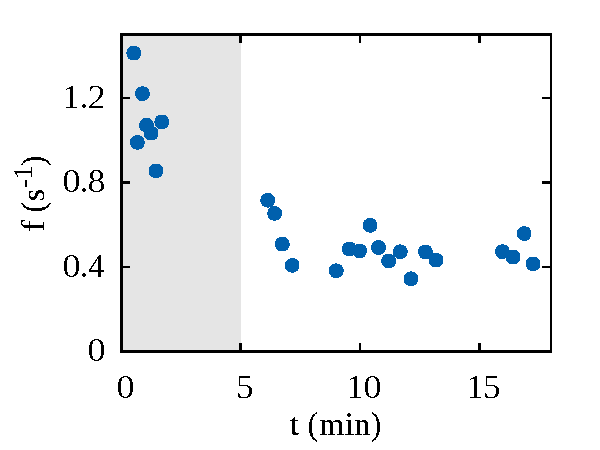
\includegraphics[width=\linewidth]{freqvst.pdf}
%    \caption{Frequency of oscillation vs. time. Grayed out area is the transient phase during which excess CA present on the surface of the cboat.}
%    \label{fig:freqvst}
%\end{figure}
%\begin{figure*}[ht]
%	\centering
%	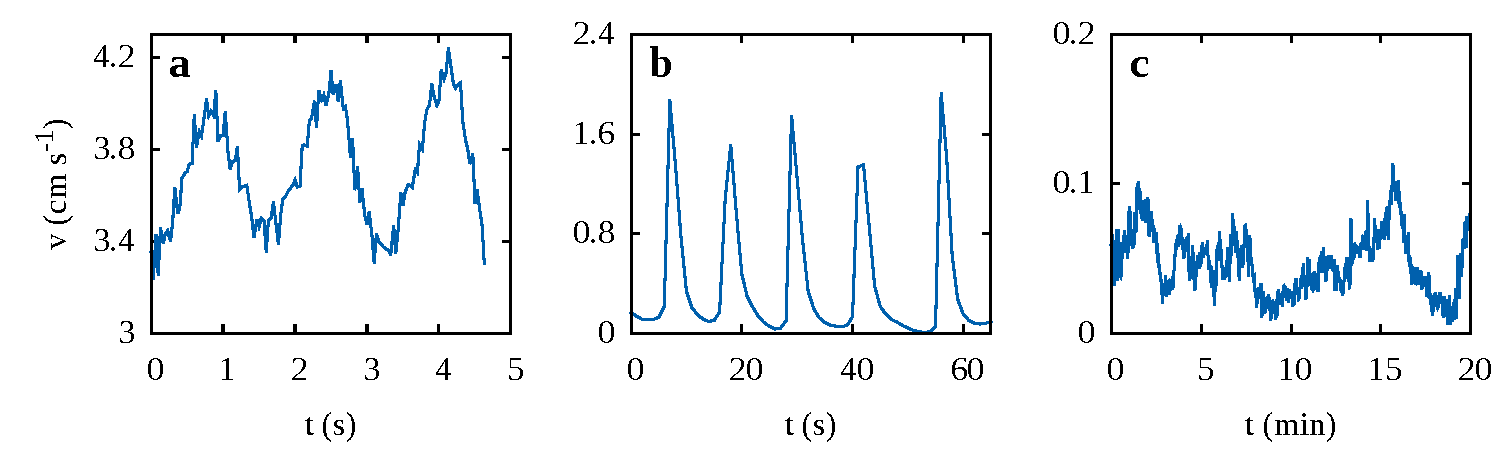
\includegraphics[width=\textwidth]{uvst_sigma.pdf}
%	\caption{{\bf (a)} at $\sigma = 72\ \mathrm{dy\ cm^{-1}}$, {\bf (b)} at $\sigma = 65\ \mathrm{dy\ cm^{-1}}$, {\bf (c)} at $\sigma = 59\ \mathrm{dy\ cm^{-1}}$}
%\label{fig:uvst_sigma}
%\end{figure*}

\section{Model}
\label{modelsec}

Let $v(t)$ be the velocity of the camphor boat, and $k(t)$ be the imbalanced surface tension gradient force acting on it because of the anisotropic distribution of camphoric acid on the interface around the c-boat.
We model the rate of change of these variable through a system of coupled ordinary different equations that qualitatively represent the essence of the underlying fluid dynamics and transport.
This system is given by
\begin{align}
\ddt{v} &= -\alpha v |v| + \beta k \label{eqn:dvdt} \\
\ddt{k} &= \gamma v + \delta k -\mu k^3, \label{eqn:dkdt}\\
\end{align}
where $\alpha$, $\beta$, $\gamma$, $\delta$ and $\mu$ are phenomenological parameters, whose significance we explain next.
Equation \eqref{eqn:dvdt} represents the Newton's second law of motion for the c-boat; the left hand side of this equation is the acceleration of the c-boat, and the right hand side includes the fluid drag and the imbalanced Marangoni force term. The fluid drag is assumed to be quadratic arising from form drag on the c-boat as the Reynolds number is O(100), and to act against the instantaneous velocity. The phenomenological coefficient $\alpha$ represents the combined effect of the coefficients parametrizing the form drag and the mass of the c-boat. The Marangoni force, as per our assumption is $k$, and therefore appears in this equation directly with the coefficient $\beta$ which represents the reciprocal of the c-boat mass.
Equation \eqref{eqn:dkdt} is also structured to represent some elementary expectations from the c-boat dynamics. The right hand side of this equation also represents the hydrodynamic influence due to the motion of the c-boat through the term proportional to $\gamma$, and the expected Marangoni force set up in the absence of any surrounding flow through the terms proportional to $\delta$ and $\mu$. The $k$-dependent terms on the right hand side are constructed such that in the absence of any c-boat motion, an asymmetric surface tension field builds up spontaneously around the c-boat on a time scale $1/\delta$, and saturates to a value $\pm\sqrt{\delta/\mu}$. The $\pm$ sign signals the spontaneous symmetry breaking in this process.

Apart from the trivial fixed point $k=v=0$, other fixed points of this dynamical system satisfy
\begin{align}
&k = \dfrac{\alpha v |v|}{\beta}, \\
&\gamma + \delta \dfrac{\alpha}{\beta} |v| - \mu \dfrac{\alpha^3}{\beta^3} v^2 |v|^3 = 0.
\end{align}
These two roots correspond to the c-boat moving in either positive or negative direction with constant speed. The term $\sqrt{\delta/\mu}$ is then analogous to the surface tension difference between CA and the ambient environment. Controlling this parameter is tantamount to the experimental condition of controlling  surface tension difference via metered dosage of SDS. 

\section{Discussion}
\label{discussec}

\section{Summary}
\label{summarysec}
TBD


{\bf Acknowledgments}\\
VSA, DKS, and MMB were supported by the Collective Interactions Unit, OIST. VSA acknowledges helpful discussions with Pinaki Chakraborty. MMB ackowledges L. Mahadevan for introducing the camphor boat system and scientific discussions, and D. Vu Anh for help with preliminary experiments. The authors acknowledge Kenneth Meacham III for experimental support and Prof. Amy Shen for help with tensiometry. 

\bibliography{CBoat}
%\bibliography{rsc} %your .bib file
\bibliographystyle{rsc} %the RSC's .bst file

%\begin{thebibliography}{}
%\bibitem{LiquidBook} J.-P. Hansen and I. R. McDonald, {\it Theory of Simple Liquids}, Academic Press, (2006).
%\bibitem{SolidBook} C. Kittel, {\it Introduction to Solid State Physics}, Wiley, (2004).
%\bibitem{effort1} M. D. Ediger, {\it Annu. Rev. Phys. Chem.} {\bf 51}, 99 (2000).
%\bibitem{effort2} E. R. Weeks, J. C. Crocker, A. C. Levitt, A. Schofield, and D. A. Weitz, {\it Science} {\bf 287}, 627 (2000).
%\bibitem{effort3} L. Berthier and G. Biroli, {\it Rev. Mod. Phys.} {\bf 83}, 587 (2011).
%\bibitem{effort4} P. J. Lu and D. Weitz, {\it Annu. Rev. Condens. Matter Phys.} {\bf 4}, 217 (2013).
%\bibitem{DH1} P. G. Wolynes, V. Lubchenko, {\it Structural Glasses and Supercooled Liquids: Theory, Experiment, and Applications} John Wiley \& Sons, (2012).
%\bibitem{DH2} L. Berthier, G. Biroli, J.-P. Bouchaud, L. Cipelletti, W. van Saarloos {\em ed.}, {\it Dynamical Heterogeneities in Glasses, Colloids, and Granular Media} Oxford University Press, (2011).
%\bibitem{conf1} J. R. Bordin, A. B. de Oliveira, A. Diehl and M. C. Barbosa, {\it J. Chem. Phys.} {\bf 137}, 084504 (2012).
%\bibitem{conf2} L. B. Krott and M. C. Barbosa, {\it J. Chem. Phys.} {\bf 138}, 084505 (2013).
%\bibitem{cell} D. Holcman and Z. Schuss, {\it J. Phys. A: Math. Theor.} {\bf 47}, 173001 (2014).
%\bibitem{aggrgt1} J. Groenewold and W. K. Kegel, {\it J. Phys. Chem. B} {\bf 105}, 11702 (2001).
%\bibitem{aggrgt2} G. Malescio and G. Pellicane, {\it Nat. Mater.} {\bf 2}, 97 (2003).
%\bibitem{aggrgt3} F. Sciortino, S. Mossa, E. Zaccarelli, and P. Tartaglia, {\it Phys. Rev. Lett.} {\bf 93}, 055701 (2004).
%\bibitem{expt1} A. Stradner, H. Sedgwick, F. Cardinaux, W. C. K. Poon, S. U. Egelhaaf, and P. Schurtenberger, {\it Nature} {\bf 432}, 492 (2004).
%\bibitem{expt2} T. H. Zhang, J. Klok, R. H. Tromp, J. Groenewolda, and W. K. Kegel, {\it Soft Matter} {\bf 8}, 667 (2012).
%\bibitem{ps1} M. Carpineti, and M. Giglio, {\it Phys. Rev. Lett.} {\bf 86} 3327 (1992).
%\bibitem{ps2} M. Muschol, and F. Rosenberger, {\it J. Chem. Phys.} {\bf 107}, 1953 (1997).
%\bibitem{arrest} P. Segre, V. Prasad, A. Schofield, and D. Weitz, {\it Phys. Rev. Lett.} {\bf 86}, 6042 (2001).
%\bibitem{neqhet1} A. M. Kulkarni, N. M. Dixit, and C. F. Zukoski, {\it Faraday Discuss.} {\bf 123}, 3 (2003).
%\bibitem{neqhet2} A. M. Puertas, M. Fuchs, and M. E. Cates, {\it J. Chem. Phys.} {\bf 121}, 2813 (2004).
%\bibitem{dbt1} D. A. Weitz, and M. Oliveria {\it Phys. Rev. Lett.} {\bf 52} 1433 (1984).
%\bibitem{dbt2} D. A. Weitz, J. S. Huang, M. Y. Lin, J. Sung {\it Phys. Rev. Lett.} {\bf 54} 1416 (1985).
%\bibitem{dbt3} G. Foffi, C. De Michele, F. Sciortino, and P. Tartaglia {\it Phys. Rev. Lett.} {\bf 94} 078301 (2005).
%\bibitem{dbt4} B. Ruzicka, E. Zaccarelli, L. Zulian, R. Angelini, M. Sztucki, A. Moussa�d, T. Narayanan, and F. Sciortino, {\it Nature materials} {\bf 10}, 56 (2011).
%\bibitem{dbt5} E. Zaccarelli, P. J. Lu, F. Ciulla, D. A. Weitz, and F. Sciortino {\it J. Phys. Condens. Matter} {\bf 20} 494242 (2008).
%\bibitem{dbt6} J. C. F. Toledano, F. Sciortino, E. Zaccarelli {\it Soft Matter} {\bf 5}, 2390 (2009).
%\bibitem{dbt7} F. Cardinaux, E. Zaccarelli, A. Stradner, S. Bucciarelli, B. Farago, S. U Egelhaaf, F. Sciortino, and P. Schurtenberger {\it J. Phys. Chem. B} {\bf 115}, 7227 (2011)
%\bibitem{glss1} E. Zaccarelli, G. Foffi, K. A. Dawson, S. V. Buldyrev, F. Sciortino, and P. Tartaglia, {\it Phys. Rev. E} {\bf 66}, 041402 (2002).
%\bibitem{glss2} N. Gnan, G. Das, M. Sperl, F. Sciortino, and E. Zaccarelli, {\it Phys. Rev. Lett.} {\bf 113}, 258302 (2014).
%\bibitem{lebo_pen} J. L. Lebowitz, O. Penrose, {\it J. Math. Phys.} {\bf 7}, 98 (1966);
%\bibitem{compint} J. L. Lebowitz, {\it Ann. Rev. Phys. Chem.} {\bf 19}, 389 (1968).
%\bibitem{colloid1} P. J. Lu, E. Zaccarelli, F. Ciulla, A. B. Schofield, F. Sciortino and D. A. Weitz, {\it Nature}, {\bf 453}, 499 (2008).
%\bibitem{protein1} R.P. Sear {\it J. Chem. Phys.} {\bf 111}(10) 4800 (1999).
%\bibitem{protein2} A. Shukla, E. Mylonas, E. Di Cola, S. Finet, P. Timmins, T. Narayanan, and D. I. Svergun, {\it Proc. Natl. Acad. Sci.} {\bf 105}, 5075 (2008).
%\bibitem{dna_np} S. Srivastava, D. Nykypanchuk, M. Fukuto, J. D. Halverson, A. V. Tkachenko, K. G. Yager, and O. Gang, {\it J. Am. Chem. Soc.} {\bf 136}, 8323 (2014).
%\bibitem{salt} C. N. Likos, {\it Physics Reports} {\bf 348} 267 (2001).
%\bibitem{globprot} G. A. Vliegenthart and H. N. W. Lekkerkerker, {\it J.Chem.Phys.} {\bf 112} (12) 5364 (2000).
%\bibitem{colloid2} A. Puertas, C. De Michele, F. Sciortino, P. Tartaglia and E. Zaccarelli {\it J. Chem. Phys.} {\bf 127} 144906 (2007).
%\bibitem{2n-n} G. A. Vliegenthart, J. M. F. Lodge, and H. N. W. Lekkerkerker, {\it Physica A} {\bf 263} 378 (1999).
%\bibitem{2Dmorph} T. Das, T. Lookman, and M. M. Bandi, {\it Soft Matter} DOI:10.1039/C5SM01222H (2015).
%\bibitem{lammps} Available at \texttt{http://lammps.sandia.gov}
%\bibitem{langevin} T. Schneider and E. Stoll, {\it Phys. Rev. B} {\bf 17}, 1302 (1978).
%\bibitem{critical} P. Charbonneau and D.R. Reichman, {\it Phys. Rev. E} {\bf 75}(5) 050401 (2007).
%\bibitem{nergo1} D. Thirumalai, R. D. Mountain, and T. R. Kirkpatrick, {\it Phys. Rev. A} {\bf 39}, 3563 (1989).
%\bibitem{nergo2} R. D. Mountain and D. Thirumalai, {\it J. Phys. Chem.} {\bf 93}, 6975 (1989).
%\bibitem{msd} S. Havlin and D. Ben-Avraham, {\it Advances in Physics} {\bf 51} 187 (2002).
%\bibitem{sfd} S. Herrera-Velarde, A. Zamudio-Ojeda, and R. Castaneda-Priego {\it J. Chem. Phys.} {\bf 133}, 114902 (2010).
%\bibitem{ovrlp1} G. Parisi, {\it J. Phys. A: Math. Gen.} {\bf 30}, L765 (1997).
%\bibitem{ovrlp2} S. C. Glotzer, V. N. Novikov, and T. B. Schroder {\it J. Chem Phys.} {\bf 112}, 509 (200)
%\bibitem{vH} L. van Hove, {\it Phys. Rev.} {bf 95} 249 (1954).
%\bibitem{nnGs} B. Wang, J. Kuo, S. C. Bae and S. Granick, {\it Nature Materials} {\bf 11}, 483 (2012).
%\bibitem{dynLnd} K. Zahn, R. Lenke, and G. Maret, {\it Phys. Rev. Lett.} {\bf 82} 2721 (1999).
%\bibitem{paretolaw} M. E. J. Newman, {\it Contemporary Physics} {\bf 46}, 323?351 (2005).
%\bibitem{enskog} S. Chapman and T.G. Cowling, The Mathematical Theory of Non-Uniform Gases (Cambridge University Press, London, 1970).
%\bibitem{exS1}R .E. Nettleton and M. S. Green, {\it J. Chem. Phys.} {\bf 29} 1365 (1958).
%\bibitem{exS2} A. Baranyai and D.J. Evans, {\it Phys. Rev. A} {\bf 40} 3817 (1989).
%\bibitem{rosenfeld} Y. Rosenfeld, {\it Phys. Rev. A} {\bf 15}, 2545-2549 (1977).
%\bibitem{dzugutov} M. Dzugutov, {\it Nature} {\bf 381}, 137 (1996).
%\bibitem{tong} X. Ma, W. Chen, Z. Wang, Y. Peng, Y. Han, and P. Tong, {\it Phys. Rev. Lett.} {\bf 110}, 078302 (2013).
%\bibitem{hoyt} J. Hoyt, M. Asta, and B. Sadigh, {\it Phys. Rev. Lett.} {\bf 85}, 594-597 (2000).
%\end{thebibliography}


\end{document}

